\section{Thin QR factorization with Householder reflectors}
Inside this section we will first introduce QR factorization and Householder reflectors, then we will talk about how to solve our task with the thin variant of the former and , finally, just like we did for the L-BFGS method, we will analyze its performances.

\subsection{Overview on thin QR factorization}
For any matrix $A \in \mathbb{R}^{m\times n}$ there exist $Q \in \mathbb{R}^{m\times m}$ orthogonal and $R \in \mathbb{R}^{m\times n}$ upper triangular such that
\begin{equation}
    A=QR
    \label{eq:qr}
\end{equation}
By diving into our case, we must introduce the thin variant of \eqref{eq:qr}. Given that $\hat{X}\in \mathbb{R}^{m\times n}$, then $R$ has the following structure
\begin{center}
$\begin{bmatrix}
r_{1,1} & r_{1,2} & r_{1,3} & \dots & r_{1,n-1} & r_{1,n} \\
0 & r_{2,2} & r_{2,3} & \dots & r_{2,n-1} & r_{2,n} \\
0 & 0 & r_{3,3} & \dots & r_{3,n-1} & r_{3,n} \\
\vdots & & & & & \vdots \\
0 & 0 & 0 & \dots & r_{n-1,n-1} & r_{n-1,n} \\
0 & 0 & 0 & \dots & 0 & r_{n,n} \\
0 & 0 & 0 & \dots & 0 & 0 \\
\vdots & & & & & \vdots \\
0 & 0 & 0 & \dots & 0 & 0 \\
\end{bmatrix}$
\end{center}
Hence, $R$ can be split into two parts where the first one is $R_1\in \mathbb{R}^{n\times n}$ and, following the same reasoning, $Q$ is split into $Q_1 \in \mathbb{R}^{m\times n}$ and $Q_2 \in \mathbb{R}^{(m-n)\times n}$. Therefore, by looking at \eqref{eq:qr} and taking into account what we said just before, $\hat{X}$ can be factorized as following
\begin{equation}
    \hat{X}=QR=
    \begin{bmatrix}Q1 & Q2\end{bmatrix}\begin{bmatrix}R1 \\ 0\end{bmatrix}=Q_1 R_1
    \label{eq:qr_factorization}
\end{equation}
Before we discuss how to solve the LLS with the assigned method we need to introduce the Householder reflectors. The QR factorization, and its thin variant, can be obtained by storing the so called Householder reflectors instead of computing Q at each step, so let $x\in \mathbb{R}^n$ be any vector and let $u\in \mathbb{R}^n$ be the normalized Householder vector of $x$ such that
\begin{subequations}
    \begin{equation}
        \label{eq:householder_u}
        u=\frac{v}{\lVert v\rVert}
    \end{equation}
    where
    \begin{equation}
        \label{eq:householder_v}
        v=\begin{bmatrix}
        x_1 - \lVert x \rVert \\
        x_2 \\
        x_3 \\
        \vdots \\
        x_{n-1} \\
        x_n
        \end{bmatrix}
    \end{equation}
\label{eq:householder_vector}
\end{subequations}
\vspace{3mm}

\noindent The Householder vector defined in \eqref{eq:householder_u} is computed by algorithm\eqref{algorithm:householder_v}

\begin{algorithm}[H]
    \caption{Householder vector}
    \label{algorithm:householder_v}
    s = $\lVert x \rVert$; \\
    \If{$x(1) \geq 0$}{s=-s;}
    v = x; \\
    v(1) = v(1) - s; \\
    u = v / $\lVert v \rVert$; \\
    \Return{u, s};
\end{algorithm}

\noindent The Householder reflector of $u$ is then defined as
\begin{equation}
    H_u=I-2uu^T
    \label{eq:householder_reflector}
\end{equation}
Householder reflectors are essential for computing the QR factorization without needing to formulate Q. More formally, given a matrix $\hat{X} \in \mathbb{R}^{m \times n}$, the algorithm we have to use consists in building a list of Householder reflectors (as defined in \eqref{eq:householder_reflector}) that transform $\hat{X}$ into an un upper triangular matrix $R \in \mathbb{R}^{m \times n}$ and in storing their products as the orthogonal matrix $Q \in \mathbb{R}^{m \times m}$.

\subsection{Solving LLS with thin QR} \label{subsec:lls_qr}
Starting from \eqref{eq:qr_factorization}, we can write
\begin{equation}
\begin{aligned}
    \lVert \hat{X}w-\hat{y} \rVert &\stackrel{\footnotemark}{=} \lVert Q^T(\hat{X}w-\hat{y}) \rVert = \lVert Q^T\hat{X}w-Q^T\hat{y} \rVert = \lVert Q^TQRw-Q^T\hat{y} \rVert = \lVert Rw-Q^T\hat{y} \rVert \\
    &= \lVert \begin{bmatrix}R_1 \\ 0 \end{bmatrix}w-\begin{bmatrix}Q_1 & Q_2\end{bmatrix}^T\hat{y} \rVert = \lVert \begin{bmatrix}R_1w \\ 0 \end{bmatrix}-\begin{bmatrix}Q_1^T\hat{y} \\ Q_2^T\hat{y}\end{bmatrix}^T\rVert = \lVert \begin{bmatrix}R_1w - Q_1^T\hat{y} \\ Q_2^T\hat{y} \end{bmatrix} \rVert
\end{aligned}
\end{equation}
\footnotetext{Holds since $\lVert Qx \rVert=\lVert x \rVert$ when $Q$ is orthogonal.}
\noindent where $R_1$ and $Q_1$ are the matrices as seen in \eqref{eq:qr_factorization} and $Q_2^T\hat{y}$ is the residual of the norm, that is the optimum of our optimization problem.
\vspace{3mm}

\noindent Moreover, from the theory is known that if a matrix is factorized as in \eqref{eq:qr_factorization} and has full column rank, then the solution of LLS is given by
\begin{subequations}
    \begin{equation}
        w=R_{1}^{-1}Q_{1}^{T}\hat{y}
        \label{eq:thin_qr_solution_1}
    \end{equation}
    by stating that
    \begin{equation}
        c=Q_1^T\hat{y}
        \label{eq:thin_qr_rewrite_c}
    \end{equation}
    then \eqref{eq:thin_qr_solution_1} can be rewritten as
    \begin{equation}
        R_1w=c
        \label{eq:thin_qr_solution_2}
    \end{equation}
\label{eq:thin_qr_solution}
\end{subequations}
\vspace{3mm}

\noindent Therefore, solving the LLS problem with QR factorization is the same as solving the linear system \eqref{eq:thin_qr_solution_2}, which is an extremely easy task once $R_1$ and $Q_1$ are computed.
We now show algorithm \ref{algorithm:compute_thin_QR} that computes the thin QR factorization, without storing the Householder matrices and keeping in memory only the $m \times n$ strictly needed elements of the $Q_1$ matrix at each step. We will not show the part that solves the upper triangular system as defined by \eqref{eq:thin_qr_solution_2} since it is not relevant to the aim of this section.

\begin{algorithm}[H]
    \caption{Compute thin $QR$ factorization}
    \label{algorithm:compute_thin_QR}
    Given $A \in R^{m \times n}$\\
    $Q_{1}y = y$\\
    \For{$j = 1$ to $min(m-1,n)$}{
        $[u, s] = householder\_vector(A[j:end, j]); \triangleright$ \textbf{\autoref{algorithm:householder_v}} \\
        $A[j,j] = s;$\\
        $A[j+1:end,j] = 0;$\\
        $A[j:end,j+1:end] = A[j:end,j+1:end] - 2u*(u^T*A[j:end,j+1:end]);$\\
        $Q_{1}y[j: end] = Q_{1}y[j:end] - 2u*(u^T*Q_{1}y[j:end]);$
    }
    $R_1=A[1:n,:];$\\
    $Q_{1}y = Q_{1}y[1:n];$ \\
    \Return{$Q_{1}y, R_1$};
\end{algorithm}

\noindent As you may notice our implementation is not a strict thin qr factorization since we do not even store $Q1$, instead at each step we compute the product $Q*\hat{y}$ considering only the affected rows starting from the j-th one. Both $Q*\hat{y}$ and $R$ are computed in the main loop from \autoref{algorithm:compute_thin_QR}, keep in mind that $Q_1\hat{y}$ and $R_1$ are taken from the first n rows of $Q*\hat{y}$ and the starting matrix respectively at the end of the computation.
\vspace{3mm}

\noindent $Q*\hat{y}$ is computed as
\begin{equation}
    Q\hat{y}=H_n\dots H_1\hat{y}
    \label{eq:thin_qr_Qy}
\end{equation}

\noindent By following the definition of Householder reflector from \eqref{eq:householder_reflector}, we can see \eqref{eq:thin_qr_Qy} as
\begin{equation}
    Q\hat{y}=(I-2u_nu_n^T)\dots (I-2u_1u_1^T)\hat{y}
    \label{eq:thin_qr_Qy_reflectors}
\end{equation}

\noindent For a single iteration, \eqref{eq:thin_qr_Qy_reflectors} can be rewritten in a more easier way
\begin{equation}
    Q_i\hat{y}=(I-2u_iu_i^T)Q_i\hat{y}=Q_i\hat{y} - 2u_i(u_i^TQ_i\hat{y})
    \label{eq:thin_qr_Qy_iteration}
\end{equation}

\noindent The same reasoning can be applied to $R$
\begin{equation}
    R=H_n\dots H_1\hat{X}
    \label{eq:thin_qr_R}
\end{equation}

\noindent Without explaining again the same process seen in \eqref{eq:thin_qr_Qy_reflectors}, we can see a single iteration for computing R as
\begin{equation}
    R_i=(I-2u_iu_i^T)R_i=R_i - 2u_i(u_i^TR_i)
    \label{eq:thin_qr_R_iteration}
\end{equation}

\noindent \eqref{eq:thin_qr_Qy_iteration} and \eqref{eq:thin_qr_R_iteration} are dimensionally feasible since we operate on submatrices of $Q*y$ and $R$ as we can see from \autoref{algorithm:compute_thin_QR} (row $7$ and $8$). To give a reason on why this is more efficient, for $R$ this means doing a product between matrices of size
\begin{subequations}
    \begin{equation}
        \mathbb{R}^{(m-i)\times 1}\times (\mathbb{R}^{1\times (m-i)} \times \mathbb{R}^{(m-i)\times (n-i)})
        \label{eq:compute_R_efficient}
    \end{equation}
    instead of doing a product between two matrices of size
    \begin{equation}
        \mathbb{R}^{(m-i)\times (m-i)}\times \mathbb{R}^{(m-i)\times (n-i)}
        \label{eq:compute_R_not_efficient}
    \end{equation}
    \label{eq:compute_R}
\end{subequations}

\noindent By following \eqref{eq:compute_R_efficient} we avoid doing any product between matrices improving the execution time of our implementation, since such product requires one more order of magnitude with respect to products between vectors, hence our choice.
\vspace{3mm}

\noindent The same reasoning, of course, can be applied to $Q*\hat{y}$ where we compute products of matrices of size
\begin{equation}
    \mathbb{R}^{(m-i)\times 1}\times (\mathbb{R}^{1\times (m-i)} \times \mathbb{R}^{(m-i)\times 1})
    \label{eq:compute_Qy_efficient}
\end{equation}
    
\noindent In this way we do not need to compute $Q_1$ and then multiplying it by $\hat{y}$, instead their product is computed step by step inside the main loop of \autoref{algorithm:compute_thin_QR}.

\paragraph{Complexity}
Analyzing the computational cost of \autoref{eq:thin_qr_solution}, we notice that the vector-matrix multiplication $Q_{1}^{T}\hat{y}$ requires $\mathcal{O}(mn)$ operations, plus the time to solve the triangular system $R_1 w = Q_{1}^{T}\hat{y}$, that is $\mathcal{O}(n^2)$. Anyway, the time spent to compute this part is lower than the one required to compute the matrices $Q_1$ and $R_1$, which is $\mathcal{O}(mn^2)$.

\subsection{Backward stability}
We know aim to show the backward stability of the QR factorization (the same reasoning applies to the thin version), by first recalling the upper bound on the relative error for the LLS as we can see from \eqref{eq:upper_bound_error}
\begin{equation}
    \frac{\lVert \Tilde{w}-w \rVert}{\lVert w \rVert} \leq u
    \label{eq:upper_bound_error}
\end{equation}
where $w$ is any number and the actual solution to $\hat{X}w-\hat{y}=0$, $\Tilde{w}$ is the perturbed solution of such problem and $u$ is the so called machine precision $2^{-52}=10^{-16}$.
\vspace{3mm}

\noindent Assume that an algorithm is used to find $\hat{y}=f(w)$, we know that due to the machine precision (which is an hardware limitation) we will not get such perfect results, instead we will obtain a perturbed value $\Tilde{y}=f(\Tilde{w})$ that, in turn, will define
\begin{subequations}
    \begin{equation}
        \Delta_{\hat{y}}=\Tilde{y}-\hat{y}
        \label{eq:forward_error}
    \end{equation}
    as the forward error and
    \begin{equation}
        \Delta_w=\Tilde{w}-w
        \label{eq:backward_error}
    \end{equation}
    as the backward error.
    \label{eq:forward_backward_error}
\end{subequations}
\vspace{3mm}

\noindent Recall also that an algorithm is called backward stable if the relative backward error from \eqref{eq:backward_error} is stable, formally
\begin{equation}
    \frac{\lVert \Tilde{w}-w \rVert}{\lVert w \rVert}=\mathcal{O}(u)
    \label{eq:backward_error_stability}
\end{equation}

\noindent We first notice that doing a product with an orthogonal matrix $Q$ is backward stable, since the product $Q\circ A = Q*A+E$ (given any matrix $A^{m\times n}$) has forward error $E$ whose norm is
\begin{equation}
    \lVert E \rVert \leq \mathcal{O}(u)\lVert Q \rVert \lVert A \rVert = \mathcal{O}(u) \lVert A \rVert
    \label{eq:forward_error_norm}
\end{equation}

\noindent moreover $Q\circ A=Q(A+Q^{-1}E)$ defines the backward error $\Delta_A=Q^{-1}E$ whose norm is
\begin{equation}
    \lVert \Delta_A \rVert \leq \lVert Q^{-1} \rVert \lVert E \rVert = \mathcal{O}(u) \lVert A \rVert
    \label{eq:backward_error_norm}
\end{equation}

\noindent With \eqref{eq:forward_error_norm} and \eqref{eq:backward_error_norm} it's easy to show that the QR factorization is backward stable by perturbing $A$ with $\Delta_A$ such that $\Tilde{Q}\Tilde{R}=qr(A+\Delta_A)$. Recall that QR factorization is made up of steps as follows
\begin{equation}
    Q_k A_{k-1} = A_k
    \label{eq:qr_stability_step}
\end{equation}

\noindent considering machine precision $u$, each step starts with $\Tilde{A}_{k-1}$ (which contains even the previous errors) and produces $\Tilde{A}_k$, each single step is backward stable since the computed $\Tilde{A}_k$ and $\Tilde{u}_k$ satisfy the perturbed version of \eqref{eq:qr_stability_step}
\begin{equation}
    \Tilde{Q}_k (\Tilde{A}_{k-1}+\Delta_{k-1}) = \Tilde{A}_k
    \label{eq:qr_stability_step_perturbed}
\end{equation}

\noindent with the norm of the accumulated error at step $k-1$ as
\begin{equation}
    \lVert \Delta_{k-1} \rVert \leq \mathcal{O}(u)\lVert \Tilde{A}_{k-1} \rVert = \mathcal{O}(u) \lVert A \rVert
    \label{eq:qr_stability_error}
\end{equation}

\noindent Then, if we consider $n$ steps we can retrieve the exact result
\begin{equation}
    \Tilde{R} = A+\Delta_0+\Tilde{Q}_1^T\Delta_1+\Tilde{Q}_1^T\Tilde{Q}_2^T\Delta_2+\dots+\Tilde{Q}_1^T\Tilde{Q}_2^T\dots\Tilde{Q}_{n-1}^T\Delta_{n-1}
    \label{eq:qr_stability_exact_result}
\end{equation}

\noindent where each of the error terms is what we have seen in \eqref{eq:qr_stability_error}, by always keeping in mind that every computation is orthogonal.
\vspace{3mm}

\noindent Therefore, the QR factorization is backward stable and the computed Q and R are the exact results of $qr(A+\Delta)$ with $\lVert \Delta \rVert \leq \mathcal{O}(u) \lVert A \rVert$.
\vspace{3mm}

\noindent Moreover, while going back to our case, backward stable algorithms usually produces small residuals $r=\hat{X}w-\hat{y}$, but this does not imply that $\Tilde{w}$ is close to the actual solution $w$ as we have seen in \ref{subsec:lbfgs_analysis}. Even then is still possible to find an upper bound to such error as theorem \ref{theorem:qr_upper_bound_error} states.
\begin{theorem}
    Let $\hat{X}=Q_1R_1$ be a thin QR factorization and let $r_1=Q_1^T(\hat{X}\Tilde{w}-\hat{y})$. Then, it can be proven that $\Tilde{w}$ is the exact solution of the least square problem
    \begin{equation}
        min \lVert \hat{X}w-(\hat{y}+Q_1r_1) \rVert
        \label{eq:qr_least_square}
    \end{equation}
    thus
    \begin{equation}
        \frac{\lVert \Tilde{w}-w\rVert}{\lVert w\rVert}\leq \kappa_{rel}(LS,\hat{y})\frac{\lVert Q_1r_1\rVert}{\lVert \hat{y} \rVert}=\kappa_{rel}(LS,\hat{y})\frac{\lVert r_1\rVert}{\lVert \hat{y} \rVert}
        \label{eq:qr_upper_bound_error}
    \end{equation}
    \label{theorem:qr_upper_bound_error}
\end{theorem}
\noindent \eqref{eq:qr_upper_bound_error} states that the relative error of the LLS problem solved with thin QR factorization is bounded by the condition number relative to such problem and by the ratio between the residual and the expected values.

\subsection{Performance analysis}
We have three different purposes for the thin QR factorization algorithm:
\begin{enumerate}
    \item we have to show that our implementation scales linearly with respect to the number of rows of the input matrix.
    \item we need to check the accuracy of our implementation.
    \item we need to show the results for varying values of $\lambda$.
\end{enumerate}

\subsubsection{Linearity of thin QR with respect to the rows}\label{subsec:qr_linearity}
The project requires us to implement a thin QR factorization algorithm that scales linearly with respect to the biggest dimension of the number of rows of a matrix, in order to prove this behavior, we created 20 $m \times n$ random matrices, with $n$ fixed and equal to 200, whereas $m$ spaces from 1000 to 5750 with a step size equal to 250. For each configuration, we ran our thin QR factorization algorithm 10 times, measuring the average completion time and then we plotted the results as shown in \autoref{fig:avg_time_qr}.
\begin{figure}[H]
    \centering
    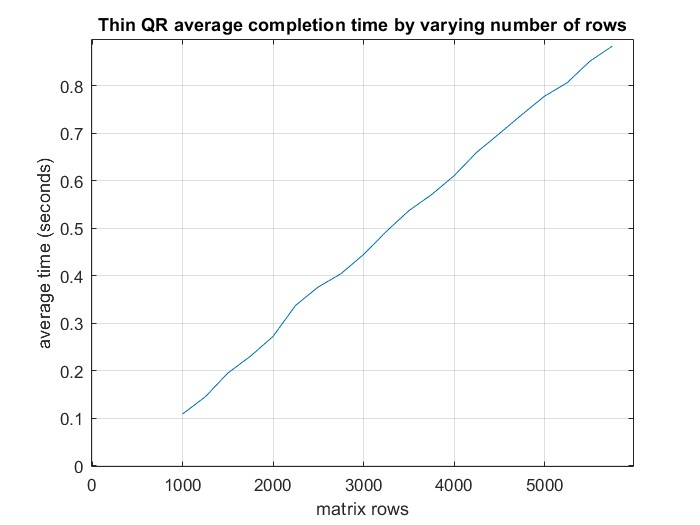
\includegraphics[width = 0.8\linewidth]{images/thin_qr/avg_time_qr.jpg}
    \caption{Thin QR average completion time by varying number of rows.}
    \label{fig:avg_time_qr}
\end{figure}

\noindent As \autoref{fig:avg_time_qr} shows, our implementation of thin QR scales linearly with the number of rows which is expected as we know that its complexity is $\mathcal{O}(mn^2)$ from the last paragraph of \ref{subsec:lls_qr}.

\subsubsection{Accuracy of thin QR}
We are also interested in the accuracy of our thin QR implementation to know how it factorizes our matrix $\hat{X}$ when $\kappa(\hat{X})$ becomes high (we already know this is caused by $\lambda$ as talked in \ref{appendix:condition_number}), such metric is defined as
\begin{equation}
    \frac{\lVert \hat{X} - Q_1R_1\rVert}{\lVert \hat{X}\rVert}
    \label{eq:thin_qr_accuracy}
\end{equation}
where $Q_1$ and $R_1$ are the matrices obtained by our thin qr factorization.
\vspace{3mm}

\noindent In short, we want to know how accurately our thin QR rebuilds the starting matrix. For such purpose, \autoref{tab:thin_qr_accuracy} shows the accuracies achieved by our method compared to the ones from the matlab implementation (called "economical thin QR") and the distance between them.
\begin{table}[H]
\centering
\begin{tabular}{c|c|c|c} \hline \hline
    $\lambda$ & Our accuracy & Matlab accuracy & $\Delta$ accuracies\\
    \hline \hline
    
    \rowcolor{gray!30} $10^4$ & $1.865168 \times 10^{-15}$ & $3.088531 \times 10^{-15}$ & $1.223363 \times 10^{-15}$ \\
    
    $10^2$ & $9.94962 \times 10^{-16}$ & $1.602198 \times 10^{-15}$ & $6.072354 \times 10^{-16}$ \\
    
    \rowcolor{gray!30} $1$ & $7.463726 \times 10^{-16}$ & $7.450506 \times 10^{-16}$ & $1.321951 \times 10^{-18}$ \\
    
    $10^{-2}$ & $7.908642 \times 10^{-16}$ & $7.630684 \times 10^{-16}$ & $2.779588 \times 10^{-17}$ \\
    
    \rowcolor{gray!30} $10^{-4}$ & $7.542911 \times 10^{-16}$ & $7.424282 \times 10^{-16}$ & $1.186286 \times 10^{-17}$ \\
    \hline \hline
\end{tabular}
\caption{Thin QR accuracy.}
\label{tab:thin_qr_accuracy}
\end{table}

\noindent From \autoref{tab:thin_qr_accuracy} we can see that our accuracy is close to $\mathcal{O}(u)=1e-16$ meaning that our implementations is, indeed, correct, as expected from a backward stable algorithm. Moreover our accuracy is extremely close to the one achieved by matlab, giving us a nice confidence boost for the next steps in this performance analysis.

\subsubsection{Results}
Since the only hyper-parameter for the thin QR is $\lambda$ we will show how the results change when the latter assumes different values, moreover we will not show the standard deviation for each configuration since it's very close to $0$ given the fact that thin QR is not iterative.
\vspace{3mm}

\noindent The considered values for $\lambda$ are the same seen in \ref{subsec:lbfgs_analysis}, but this time we consider one more metric which is the gradient of the function $\nabla f(w)$ in $w$, since we did not use it as stop condition. As for the L-BFGS, using the relative error on $w$ is fine given the fact that $w^*$ is unique, thanks to what we have seen in \ref{subsec:introduction_convexity}.
\vspace{3mm}

\noindent We also consider the upper bound from \eqref{eq:qr_upper_bound_error} since it gives us a nice information about the maximum relative error we can achieve by computing the solution using non-exact arithmetic. Moreover, \eqref{eq:qr_upper_bound_error} can be rewritten as 
\begin{equation}
    \frac{\lVert w - w^* \lVert}{\lVert w^*\rVert}\leq\kappa_{rel}(LS,\hat{y})\frac{\lVert r_1\rVert}{\lVert \hat{y} \rVert}\stackrel{\footnotemark}{=} \frac{\kappa(\hat{X})}{\lVert \hat{X}w \rVert}\lVert r_1 \rVert
    \label{eq:qr_upper_bound_performance}
\end{equation}
\footnotetext{recall that $\kappa_{rel}(LS,\hat{y})=\frac{\kappa(\hat{X})}{\cos{\theta}}$, where $\cos{\theta}=\frac{\lVert \hat{X}w \rVert}{\lVert \hat{y} \rVert}$.}

\noindent We can now show the results achieved by our implementation in \autoref{tab:thin_qr_results} before doing a brief explanation about them.
\begin{table}[H]
\centering
\begin{tabular}{c|c|c|c|c} \hline \hline
    $\lambda$ & $\frac{\lVert w - w^* \lVert}{\lVert w^*\rVert}$ & $\frac{\lVert \hat{X}w - y \lVert }{\lVert y \lVert}$ & $\lVert \nabla f(w) \lVert$ & $\frac{\kappa(\hat{X})}{\lVert \hat{X}w \rVert}\lVert r_1 \rVert$ \eqref{eq:qr_upper_bound_performance} \\ \hline \hline
    
    \rowcolor{gray!30} $10^4$ & $7.3825 \times 10^{-14}$ & $9.9959 \times 10^{-1}$& $1.8069 \times 10^{-10}$ & $1.0512 \times 10^{-13}$ \\
    
    $10^2$ & $1.5650\times 10^{-14}$ & $9.1160 \times 10^{-1}$ & $6.0329 \times 10^{-12}$ & $2.7837\times 10^{-14}$ \\
    
    \rowcolor{gray!30} $1$ & $2.0354 \times 10^{-14}$ & $5.3405 \times 10^{-2}$ & $2.7046 \times 10^{-12}$ & $1.1681\times 10^{-12}$ \\
    
    $10^{-2}$ & $9.0120 \times 10^{-14}$ & $5.4414 \times 10^{-4}$ & $4.6584 \times 10^{-12}$ & $2.0006\times 10^{-10}$ \\
    
    \rowcolor{gray!30} $10^{-4}$ & $8.1724 \times 10^{-14}$ & $5.4071 \times 10^{-6}$ & $6.1100 \times 10^{-12}$ & $1.0513\times 10^{-8}$ \\
    \hline \hline
\end{tabular}
\caption{Thin QR results. $w^{*}$ is the Matlab solution from $\hat{X} \backslash\hat{y}$.}
\label{tab:thin_qr_results}
\end{table}

\noindent The execution time is more or less $9.8s$ for each configuration so we decided not to report it. By considering the upper bound from \eqref{eq:qr_upper_bound_performance}, we can notice how it decreases as $\lambda$ increases since $\kappa(\hat{X})$ starts to get bigger and bigger. Anyway, the bound always holds for our implementation, even for small values of $\lambda$, as we expected from the theory.
\vspace{3mm}

\noindent Furthermore, we noticed that the residuals follow the same behavior as we have seen for the L-BFGS in \ref{subsec:lbfgs_analysis}, that is the decreasing of the relative residual as the value of $\lambda$ decreases.
